% Figure 1 — Overview of the late-fusion survival model (MoR Fig.1 레이아웃).
%   Left   : tabular arm 내부 (clinical MLP + RadBERT-MLP -> L2 -> concat 144 -> Cox head)
%   Middle : 전체 모델 (image arm + tabular arm -> r_img, r_tab -> fold-wise CoxPH combiner)
%   Right  : 5-fold 교차검증에서 arm 모델과 combiner 가 각각 어느 환자를 보는지 (누수 없음)
% 수치 출처: src/sclc/model.py (브랜치 구조), src/sclc/late_fusion.py (combiner),
%            data/splits/trimodal_common_5fold_seed42_v1.csv (fold 크기).
\documentclass[tikz,border=6pt]{standalone}
% 논문 그림 공통 스타일 (fig1/fig2 가 \input 한다).
% 시각 언어는 Mixture-of-Recursions(MoR) 논문 Fig.1/2 를 따른다:
%   파스텔 채움 + 진남색 얇은 윤곽 + 둥근 모서리, 산세리프 라벨.
% 색 의미(두 그림에서 동일):
%   boxblue   = 영상 모달리티      boxpurple = 임상 모달리티     boxpink = 판독지 모달리티
%   boxgray   = 일반 연산 블록     boxyellow = Cox 관련(head/combiner)
%   dashed    = 동결(frozen) 사전학습 모듈
\usepackage[T1]{fontenc}
\usepackage{helvet}
\renewcommand{\familydefault}{\sfdefault}
\usepackage{amsmath,amssymb}
\usetikzlibrary{positioning,arrows.meta,calc,fit,backgrounds}

\definecolor{navy}{HTML}{2F3B52}
\definecolor{ink}{HTML}{1A1A1A}
\definecolor{ink2}{HTML}{5A5E66}
\definecolor{boxblue}{HTML}{CFE0F7}
\definecolor{boxpink}{HTML}{F6CDD0}
\definecolor{boxpurple}{HTML}{DCD6F3}
\definecolor{boxyellow}{HTML}{FDEEB8}
\definecolor{boxgray}{HTML}{E9E9E9}
\definecolor{cellhold}{HTML}{3F5A8A}
\definecolor{cellfit}{HTML}{F8DD8A}
\definecolor{celleval}{HTML}{F2A4A8}

\tikzset{
  every node/.style={text=ink},
  blk/.style={draw=navy, line width=0.7pt, rounded corners=2.5pt, fill=#1,
              inner xsep=4pt, inner ysep=3pt, font=\footnotesize, align=center},
  blk/.default=boxgray,
  lay/.style={blk=#1, minimum width=30mm, minimum height=6mm},
  inp/.style={blk=#1, minimum width=15mm, minimum height=7mm},
  frozen/.style={lay=boxgray, dashed},
  container/.style={draw=navy, line width=0.8pt, rounded corners=6pt, fill=white, inner sep=6pt},
  armbox/.style={draw=navy, line width=0.6pt, dashed, rounded corners=5pt, inner sep=4pt},
  arr/.style={-{Latex[length=2.2mm,width=1.7mm]}, draw=navy, line width=0.75pt},
  lab/.style={font=\scriptsize, text=ink2, align=center, inner sep=1pt},
  op/.style={circle, draw=navy, line width=0.7pt, fill=white, inner sep=0pt,
             minimum size=4.2mm, font=\scriptsize},
  risk/.style={font=\footnotesize, inner sep=2pt},
  stage/.style={font=\scriptsize\itshape, text=ink2, inner sep=1pt},
  ptitle/.style={font=\footnotesize, align=center, inner sep=2pt},
}

% ---------------------------------------------------------------------------
% 입력 모달리티 아이콘 (fig2 입력단). 글자 라벨 대신 실제 PET-CT MIP 한 장 +
% 임상 표 / 판독지 문서 픽토그램을 쓴다. 모두 약 10.5mm x 12mm 로 크기를 맞추고
% 채움색은 모달리티 색(boxblue/boxpurple/boxpink), 윤곽은 navy 로 본문 도형과 통일.
%   사용: \iconimage{노드이름}{(x,y)}  등. 노드이름으로 화살표를 걸 수 있다.
\newcommand{\iconimage}[2]{%
  \node[blk=boxblue, inner sep=1.1pt, minimum width=0pt, minimum height=0pt] (#1) at #2
       {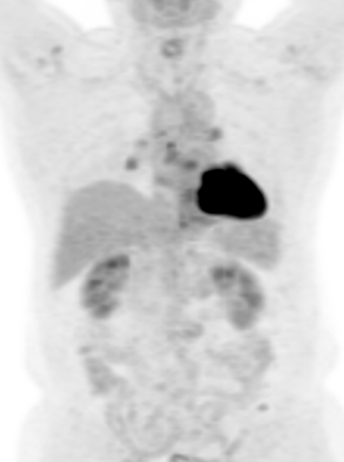
\includegraphics[height=11.8mm]{assets/pet_mip_icon.png}};%
}
\newcommand{\iconclinical}[2]{%
  \begin{scope}[shift={#2}]
    \begin{scope}
      \clip[rounded corners=2.5pt] (-5.25mm,-6mm) rectangle (5.25mm,6mm);
      \fill[boxpurple] (-5.25mm,-6mm) rectangle (5.25mm,6mm);
      \fill[navy!28]   (-5.25mm,3.3mm) rectangle (5.25mm,6mm);
      \draw[navy!45, line width=0.35pt]
        (-5.25mm,3.3mm) -- (5.25mm,3.3mm)  (-5.25mm,0.8mm) -- (5.25mm,0.8mm)
        (-5.25mm,-1.7mm) -- (5.25mm,-1.7mm) (-5.25mm,-4.2mm) -- (5.25mm,-4.2mm)
        (-1.75mm,-6mm) -- (-1.75mm,6mm)     (1.75mm,-6mm) -- (1.75mm,6mm);
    \end{scope}
    \draw[navy, line width=0.7pt, rounded corners=2.5pt] (-5.25mm,-6mm) rectangle (5.25mm,6mm);
    \node[minimum width=10.5mm, minimum height=12mm, inner sep=0pt] (#1) at (0,0) {};
  \end{scope}%
}
\newcommand{\iconreport}[2]{%
  \begin{scope}[shift={#2}]
    \fill[boxpink] (-4.6mm,-6mm) -- (-4.6mm,6mm) -- (1.7mm,6mm) -- (4.6mm,3.1mm) -- (4.6mm,-6mm) -- cycle;
    \draw[navy, line width=0.7pt, rounded corners=1pt]
      (-4.6mm,-6mm) -- (-4.6mm,6mm) -- (1.7mm,6mm) -- (4.6mm,3.1mm) -- (4.6mm,-6mm) -- cycle;
    \fill[navy!20] (1.7mm,6mm) -- (1.7mm,3.1mm) -- (4.6mm,3.1mm) -- cycle;
    \draw[navy, line width=0.55pt] (1.7mm,6mm) -- (1.7mm,3.1mm) -- (4.6mm,3.1mm);
    \draw[navy!55, line width=0.5pt]
      (-2.9mm,1.4mm) -- (2.9mm,1.4mm)  (-2.9mm,-0.4mm) -- (2.9mm,-0.4mm)
      (-2.9mm,-2.2mm) -- (2.9mm,-2.2mm) (-2.9mm,-4.0mm) -- (0.9mm,-4.0mm);
    \node[minimum width=9.2mm, minimum height=12mm, inner sep=0pt] (#1) at (0,0) {};
  \end{scope}%
}

\begin{document}
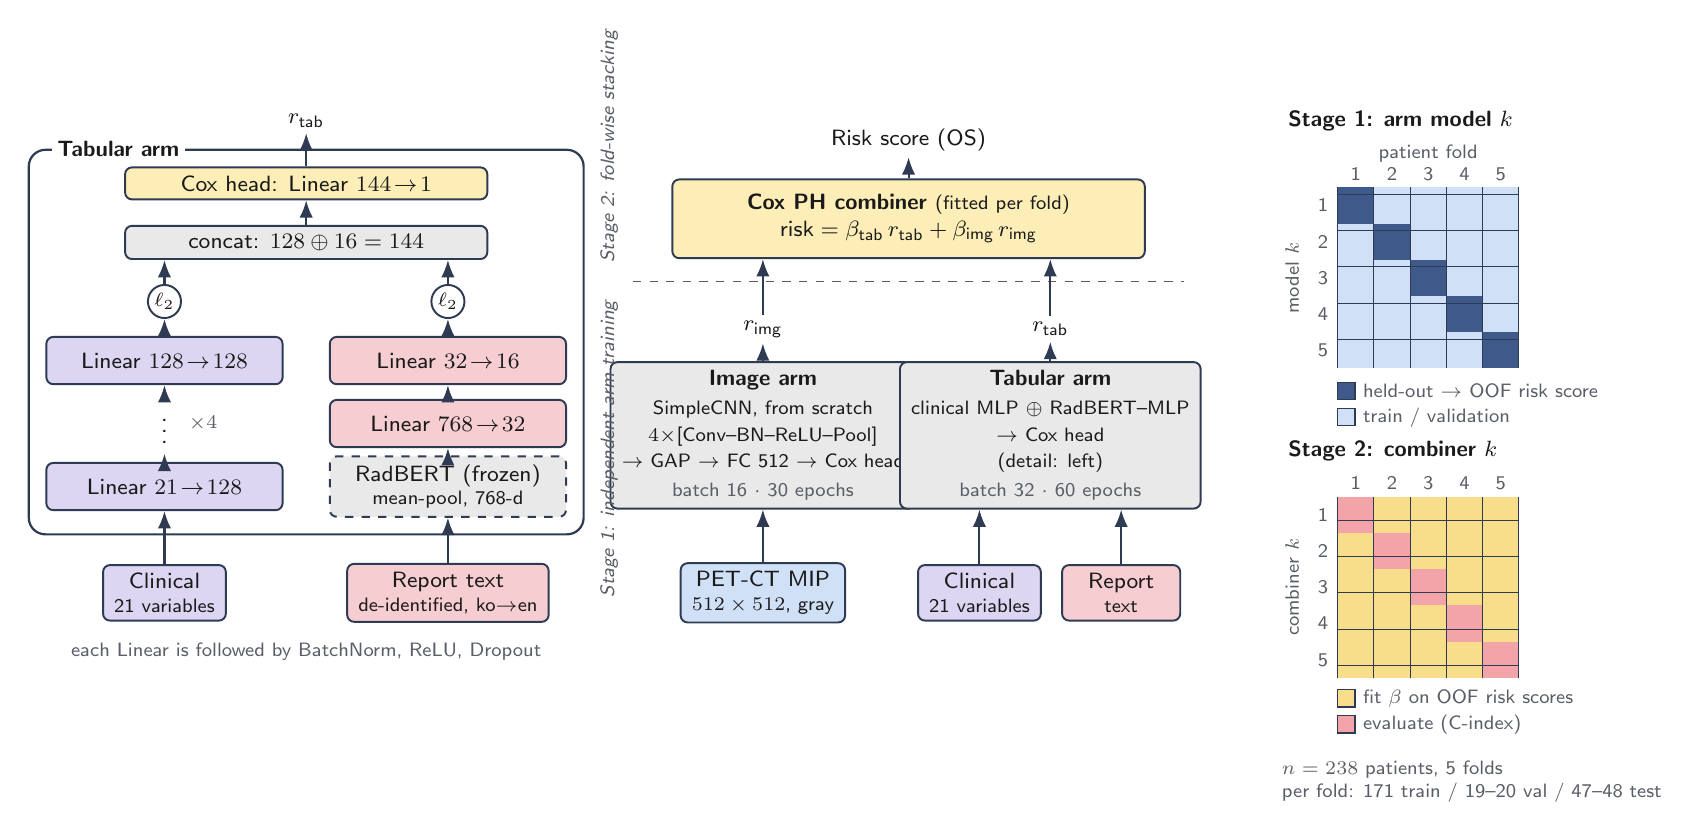
\begin{tikzpicture}[x=1cm,y=1cm]

% ===================== LEFT: tabular arm (detail) =====================
\begin{scope}[shift={(0,0)}]
  % inputs
  \node[inp=boxpurple] (xc) at (0,0)   {Clinical\\[-1pt]{\scriptsize 21 variables}};
  \node[inp=boxpink]   (xr) at (3.6,0) {Report text\\[-1pt]{\scriptsize de-identified, ko$\to$en}};
  % clinical column: Linear-BN-ReLU-Dropout x4 @128
  \node[lay=boxpurple] (c1) at (0,1.35) {Linear $21\!\to\!128$};
  \node[font=\small]   (cd) at (0,2.15) {$\vdots$};
  \node[lab, right=1mm of cd] {$\times 4$};
  \node[lay=boxpurple] (c4) at (0,2.95) {Linear $128\!\to\!128$};
  % report column: frozen RadBERT -> MLP (32,16)
  \node[frozen]        (rb) at (3.6,1.35) {RadBERT (frozen)\\[-1pt]{\scriptsize mean-pool, 768-d}};
  \node[lay=boxpink]   (r1) at (3.6,2.15) {Linear $768\!\to\!32$};
  \node[lay=boxpink]   (r2) at (3.6,2.95) {Linear $32\!\to\!16$};
  % L2 normalise, concat, Cox head
  \node[op] (l2c) at (0,3.7)   {$\ell_2$};
  \node[op] (l2r) at (3.6,3.7) {$\ell_2$};
  \node[blk, minimum width=46mm]           (cat) at (1.8,4.45) {concat: $128\oplus16=144$};
  \node[blk=boxyellow, minimum width=46mm] (hd)  at (1.8,5.2)  {Cox head: Linear $144\!\to\!1$};
  \node[risk] (rt) at (1.8,6.0) {$r_{\text{tab}}$};
  % arrows
  \draw[arr] (xc) -- (c1);   \draw[arr] (xr) -- (rb);
  \draw[arr] (c1) -- (cd);   \draw[arr] (cd) -- (c4);
  \draw[arr] (rb) -- (r1);   \draw[arr] (r1) -- (r2);
  \draw[arr] (c4) -- (l2c);  \draw[arr] (r2) -- (l2r);
  \draw[arr] (l2c.north) -- (l2c.north |- cat.south);
  \draw[arr] (l2r.north) -- (l2r.north |- cat.south);
  \draw[arr] (cat) -- (hd);  \draw[arr] (hd) -- (rt);
  % container
  \begin{scope}[on background layer]
    \node[container, fit=(c1)(rb)(hd)(l2c)(l2r)] (tab) {};
  \end{scope}
  \node[font=\footnotesize\bfseries, fill=white, inner sep=2pt, anchor=west]
        at ($(tab.north west)+(0.3,0)$) {Tabular arm};
  \node[lab] at (1.8,-0.75) {each Linear is followed by BatchNorm, ReLU, Dropout};
\end{scope}

% ===================== MIDDLE: full model =====================
\begin{scope}[shift={(7.6,0)}]
  % inputs
  \node[inp=boxblue]   (im) at (0,0)    {PET-CT MIP\\[-1pt]{\scriptsize $512\times512$, gray}};
  \node[inp=boxpurple] (cl) at (2.75,0) {Clinical\\[-1pt]{\scriptsize 21 variables}};
  \node[inp=boxpink]   (rp) at (4.55,0) {Report\\[-1pt]{\scriptsize text}};
  % arms (Stage 1)
  \node[blk, minimum width=30mm, minimum height=17mm] (ia) at (0,2.0)
        {\textbf{Image arm}\\[1pt] {\scriptsize SimpleCNN, from scratch}\\ {\scriptsize $4\times$[Conv--BN--ReLU--Pool]}\\ {\scriptsize $\to$ GAP $\to$ FC 512 $\to$ Cox head}\\[1pt] {\scriptsize\color{ink2} batch 16 $\cdot$ 30 epochs}};
  \node[blk, minimum width=32mm, minimum height=17mm] (ta) at (3.65,2.0)
        {\textbf{Tabular arm}\\[1pt] {\scriptsize clinical MLP $\oplus$ RadBERT--MLP}\\ {\scriptsize $\to$ Cox head}\\ {\scriptsize (detail: left)}\\[1pt] {\scriptsize\color{ink2} batch 32 $\cdot$ 60 epochs}};
  % OOF risk scores
  \node[risk] (ri)  at (0,3.35)    {$r_{\text{img}}$};
  \node[risk] (rtb) at (3.65,3.35) {$r_{\text{tab}}$};
  % Stage separator
  \draw[dashed, ink2, line width=0.4pt] (-1.65,3.95) -- (5.35,3.95);
  % 회전 라벨: Stage 1 은 구분선 아래로, Stage 2 는 위로 뻗게 앵커를 나눠 서로 겹치지 않게 한다.
  \node[stage, rotate=90, anchor=east] at (-1.95,3.75) {Stage 1: independent arm training};
  \node[stage, rotate=90, anchor=west] at (-1.95,4.15) {Stage 2: fold-wise stacking};
  % combiner (Stage 2)
  \node[blk=boxyellow, minimum width=60mm, minimum height=10mm] (cb) at (1.85,4.75)
        {\textbf{Cox PH combiner} {\scriptsize(fitted per fold)}\\ $\text{risk}=\beta_{\text{tab}}\,r_{\text{tab}}+\beta_{\text{img}}\,r_{\text{img}}$};
  \node[risk] (out) at (1.85,5.75) {Risk score (OS)};
  % arrows
  \draw[arr] (im) -- (ia);  \draw[arr] (cl) -- (cl |- ta.south);  \draw[arr] (rp) -- (rp |- ta.south);
  \draw[arr] (ia) -- (ri);  \draw[arr] (ta) -- (rtb);
  \draw[arr] (ri.north)  -- (ri.north  |- cb.south);
  \draw[arr] (rtb.north) -- (rtb.north |- cb.south);
  \draw[arr] (cb) -- (out);
\end{scope}

% ===================== RIGHT: cross-validation / out-of-fold stacking =====================
\begin{scope}[shift={(14.9,0)}]
  \def\cs{0.46}   % cell size (cm)
  % ---- top grid: Stage 1 arm models ----
  \node[font=\footnotesize\bfseries, anchor=south west] at (-0.75,5.75) {Stage 1: arm model $k$};
  \node[lab, anchor=south] at (2.5*\cs,5.42) {patient fold};
  \foreach \j in {1,...,5} { \node[lab, anchor=south] at ({(\j-0.5)*\cs},5.2) {\j}; }
  \foreach \i in {1,...,5} {
    \node[lab, anchor=east] at (-0.08,{5.15-(\i-0.5)*\cs}) {\i};
    \foreach \j in {1,...,5} {
      \ifnum\i=\j
        \fill[cellhold] ({(\j-1)*\cs},{5.15-\i*\cs}) rectangle ({\j*\cs},{5.15-(\i-1)*\cs});
      \else
        \fill[boxblue]  ({(\j-1)*\cs},{5.15-\i*\cs}) rectangle ({\j*\cs},{5.15-(\i-1)*\cs});
      \fi
    }
  }
  \draw[navy, line width=0.4pt] (0,{5.15-5*\cs}) grid[step=\cs] (5*\cs,5.15);
  \node[lab, rotate=90, anchor=south] at (-0.45,{5.15-2.5*\cs}) {model $k$};
  % legend
  \fill[cellhold] (0,2.45) rectangle +(0.22,0.22); \node[lab, anchor=west] at (0.28,2.56) {held-out $\to$ OOF risk score};
  \fill[boxblue]  (0,2.12) rectangle +(0.22,0.22); \node[lab, anchor=west] at (0.28,2.23) {train / validation};
  \draw[navy, line width=0.4pt] (0,2.45) rectangle +(0.22,0.22) (0,2.12) rectangle +(0.22,0.22);
  % ---- bottom grid: Stage 2 combiner ----
  \node[font=\footnotesize\bfseries, anchor=south west] at (-0.75,1.55) {Stage 2: combiner $k$};
  \foreach \j in {1,...,5} { \node[lab, anchor=south] at ({(\j-0.5)*\cs},1.27) {\j}; }
  \foreach \i in {1,...,5} {
    \node[lab, anchor=east] at (-0.08,{1.22-(\i-0.5)*\cs}) {\i};
    \foreach \j in {1,...,5} {
      \ifnum\i=\j
        \fill[celleval] ({(\j-1)*\cs},{1.22-\i*\cs}) rectangle ({\j*\cs},{1.22-(\i-1)*\cs});
      \else
        \fill[cellfit]  ({(\j-1)*\cs},{1.22-\i*\cs}) rectangle ({\j*\cs},{1.22-(\i-1)*\cs});
      \fi
    }
  }
  \draw[navy, line width=0.4pt] (0,{1.22-5*\cs}) grid[step=\cs] (5*\cs,1.22);
  \node[lab, rotate=90, anchor=south] at (-0.45,{1.22-2.5*\cs}) {combiner $k$};
  % legend
  \fill[cellfit]  (0,-1.45) rectangle +(0.22,0.22); \node[lab, anchor=west] at (0.28,-1.34) {fit $\beta$ on OOF risk scores};
  \fill[celleval] (0,-1.78) rectangle +(0.22,0.22); \node[lab, anchor=west] at (0.28,-1.67) {evaluate (C-index)};
  \draw[navy, line width=0.4pt] (0,-1.45) rectangle +(0.22,0.22) (0,-1.78) rectangle +(0.22,0.22);
  \node[lab, anchor=north west, align=left] at (-0.75,-2.1)
        {$n=238$ patients, 5 folds\\ per fold: 171 train / 19--20 val / 47--48 test};
\end{scope}

\end{tikzpicture}
\end{document}
